\newpage
\chapter{Introducción}

En 2020, el \textbf{cáncer de próstata, (Prostate Cancer, PCa)} fue el segundo tipo de cáncer más frecuente, y el quinto más mortal, en varones \cite{GlobalCancer}. Una \textbf{biopsia de próstata} es una prueba que consiste en la extracción de pequeños tejidos de la próstata para examinar posibles signos de cáncer (Ver Figura \ref{fig:biopsias_ejemplos}). El \textbf{Sistema de Puntuación de Gleason (Gleason Score)} es una calificación, en el rango de 2 a 10, que se da a biopsias de la próstata tras ser examinadas bajo un microscopio \cite{GleasonGov}. Valores más altos indican cánceres más agresivos y de crecimiento más rápido. En 2014 la \textbf{Sociedad Internacional de Patología Urológica (International Society of Urological Pathology, ISUP)} propuso un nuevo sistema basado en la Puntuación de Gleason, que propone cinco grupos ordenados (\textbf{Gleason Groups, GGs}) \cite{ISUP2014Disc}:
\begin{itemize}
\item \textbf{GG1: } Cáncer de grado bajo. Puntuación de gleason 6 o inferior.
\item \textbf{GG2: } Cáncer de grado medio. Puntuación de gleason 7.
\item \textbf{GG3: } Cáncer de grado medio pero más agresivo que GG2. Puntuación de gleason 7 pero percibido más agresivo.
\item \textbf{GG4: } Cáncer de grado alto. Puntuación de gleason 8.
\item \textbf{GG5: } Cáncer de grado alto. Puntuación de gleason 9 o 10.
\end{itemize}

\begin{figure}[H]
    \centering
    \begin{subfigure}[b]{0.3\textwidth}
        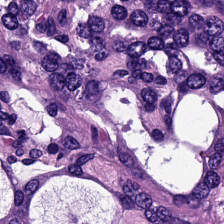
\includegraphics[width=\linewidth]{images/EjemploBiopsia1.png}
    \end{subfigure}
    \hfill
    \begin{subfigure}[b]{0.3\textwidth}
        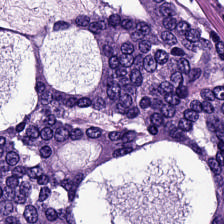
\includegraphics[width=\linewidth]{images/EjemploBiopsia2.png}
    \end{subfigure}    
    \hfill
    \begin{subfigure}[b]{0.3\textwidth}
        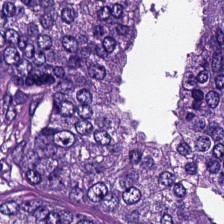
\includegraphics[width=\linewidth]{images/EjemploBiopsia3.png}
    \end{subfigure}

    \caption{Tres imágenes correspondientes a tres biopsias distintas.}
    \label{fig:biopsias_ejemplos}
\end{figure}


En el campo de la \textbf{Inteligencia Artificial (IA)}, la necesidad de asegurar transparencia y confiabilidad a dado pie a acuñar el término de \textbf{Inteligencia Artificial eXplicable (eXplainable Artificial Inteligence, XAI)} \cite{XAIManifesto}. El uso de XAI es especiamente importantes en ámbitos donde la toma de decisiones repercute directamente en la vida de las personas, como es el caso de la medicina. La Unión Europea ha propuesto una \href{https://eur-lex.europa.eu/eli/reg/2024/1689/oj}{regulación} para el uso de IA asistida en estos aspectos, entre ellos, que estos sistemas sean capaces de explicar sus decisiones de forma clara y comprensible.

Dentro del campo de la XAI, hay diferentes propuestas para la evaluación y la mejora de las explicaciones generadas. Por un lado, herramientas como \textbf{REVEL} \cite{REVEL} permiten analizar la calidad de las mismas de manera robusta. Por otro, enfoques como \textbf{X-SHIELD} \cite{XSHIELD} buscan mejorar las explicaciones mediante técnicas de regularización que aseguran el buen comportamiento de la generación de explicaciones. Aplicar estas técnicas en imagen médica puede ayudar a mejorar la interpretación de las personas profesionales de la salud de las decisiones de una IA que asista.

En este contexto este Trabajo de Fin de Máster trata de resolver el problema de \textbf{construir un modelo de IA de clasificación para lesiones cancerosas en biposias de próstata} y de la \textbf{mejora en interpretabilidad del modelo mediante técnicas de XAI}. Para esto se vamos a utilizar las herramientas REVEL y XSHIELD, y propondremos posibles mejoras de XSHIELD.


El TFM se estructura del siguiente modo. En primer lugar vamos a introducir los fundamentos teóricos necesarios para el correcto entendimiento del trabajo realizado (Capítulo \ref{cap:ft}). Después se va a hacer un estudio del estado del arte (Capítulo \ref{cap:eda}). A continuación presentamos las propuestas de este TFM (Capítulo \ref{cap:met}). En el Capítulo \ref{cap:exp} se describe el conjunto de datos con el que trabajamos, los distintos experimentos que realizamos y discutimos los resultados . Finalmente en el Capítulo \ref{cap:conc} se incluyen conclusiones y posibles trabajos futuros.


\section{Objetivos}

El objetivo principal del TFM es la utilización (y propuesta) de técnicas de evaluación y mejora de explicaciones  para modelos de clasificación de imágenes para detección de tejidos cancerosos en biopsias de próstata. Para el desarrollo del TFM, se divide el objetivo en distintos subobjetivos:

\begin{itemize}
\item Revisión del estado del arte \highlight{Cuál?}.
\item Estudio del código que implementa \cite{REVEL, XSHIELD} para su correcto entendimiento.
\item Proposición de nuevos métodos XAI para mejora de explicaciones para modelos de explicación.
\item Modificación del código para implementar dichas propuestas.
\item Diseño de los experimentos a realizar e implementación de estos.
\item Evaluación de los resultados y subsecuente discusión.
\end{itemize}

Aquí introduciría el objetivo principal del TFM y lo dividiría en algunos sub-objetivos (revisión del estado del arte, estudio de las implementaciones de las métricas ReVEL/regularización X-Shield, proposición de mis regularizaciones, implementación de estas, experimentación y finalmente evaluación/discusión de estos). 


\section{Planificación}

\highlight{
En esta sección hablo de cómo me he planificado el proyecto según estudio del problema/diseño de mis modelos/implementación/experimentación (haría una tabla). Luego haría una comparación de mi planificación vs cómo se ha repartido finalmente y haría una estimación final de cuántas horas me ha llevado el TFM y en cuánto se estima el coste del proyecto final.

POR HACER
}


\clearpage
\chapter{Fundamentos teóricos} \label{cap:ft}

En esta sección haría una introducción a la parte teórica de deep learning.

La sección de aprendizaje automático sería los fundamentos.

La sección de deep learning introduce conceptos de deep learning y en particular de visión por computador.

\textbf{Importante, justo las dos secciones anteriores las tengo ya escritas en mi TFG, que justo trata de una aplicación de visión por computador, me preguntaba si se puede reutilizar lo que tengo en mi TFG o quizás eso no es buena praxis y debería reescribirlo, estoy interesado en saberlo).}

Finalmente tendría la sección más relevante para este TFM que sería la de . Primero haría una introducción más general basándome en este paper (https://www.sciencedirect.com/science/article/pii/S1566253523001148) y luego explicaría LIME para explicar bien lo que son las métricas REVEL más adelante. 
\section{Aprendizaje automático}


\subsection{Problema de clasificación}

\subsection{Problema de regresión}

\subsection{Optimización} \label{optimización}


\subsection*{Sobreentrenamiento}



\section{Deep Learning}

\subsection*{Redes neuronales}

\subsection*{Funciones de activación}




\subsection*{Batch normalization}


\subsection*{Dropout}


\subsection{Redes convolucionales}

\subsection*{Capas convolucionales}

\subsection*{Capas de pooling}


\subsection*{Capas totalmente conectadas}


\section{XAI}

\subsection{LIME}

\subsection{Métricas ReVEL}

\subsection{Regularización X-Shield}


\newpage
\chapter{Estado del arte} \label{cap:eda}


En esta sección hago búsquedas en Scopus para ver el estado del arte y analizarlo. Para seros sinceros no tengo muy claro que debería buscar ya que dudo que encuentre artículos que apliquen explicabilidad a detección de cánceres de próstata (aunque está bien hacer la búsqueda para tenerlo claro). 

Por otro lado quizás debería buscar trabajos que traten la detección automática de cánceres de próstata o que apliquen explicabilidad a otras tareas médicas a ver que encuentro. Estoy interesado en ver cómo debería enfocar el estado del arte.

\newpage
\chapter{Métodos} \label{cap:met}
En este capítulo introduciría qué son las métricas revel en profundidad (cálculo/interpretación) + La regularización X-SHIELD. Luego introduciría mis propuestas. Antes de introducir mis propuestas haría un introducción sobre EfficientNet (en particular efficientnet b2) e introduciría su arquitectura y por qué la he elegido.

\section{Métricas ReVEL} \label{sec:FSCNet} 
\section{X-Shield} 


\clearpage
\section{Métodos propuestos} \label{sec:metodospropuestos}
\subsection{EfficientNet}
\subsection{FXShield}
\subsection{FRShield}
\subsection{HShield}

\clearpage

\section{Implementación}

Aquí explico de qué código he partido (+ GitHub), breve introducción de cómo está organizado el proyecto (en carpetas/archivos), los datos, cómo me he organizado el proyecto en conda (versión de python + modulos) finalmente pondría un link al proyecto en mi GitHub). Por cierto me interesa saber si prefieres que cree un fork de alguno de tus proyectos en github (Iván) o si me creo uno a parte en el mío (obviamente referenciando tu github como partida), a mi me da igual.



\clearpage


\newpage
\chapter{Experimentos} \label{cap:exp}


\section{Datos empleados} \label{sec:datos}
En esta sección explico el conjunto de datos del que parto. Explico como está organizado, cómo están balanceadas las clases, qué clases hay, qué significan, puedo mostrar algunos datos para mostrar ejemplos (si tengo permiso, claro). Me interesa saber de dónde provienen los datos también para ponerlo. En cuanto a estudio cualitativo de estos no creo que yo pueda aportar mucho así que no creo que haga (además de que hay demasiados datos).
\section{Experimentos realizados}

\subsection{Separación de datos}

Cómo están divididos los datos. He utilizado un conjunto de validación ya que validación cruzada es demasiado costoso en tiempo.

\paragraph*{Validation}

\paragraph*{Optimizador y elección de hiperparámetros}



\section{Métricas}
Explico que he utilizado Accurcy, cross entropy error y recuerdo el uso de la métricas revel. También hablo de los test estadísticos que he utilizado y los parámetros escogidos.
\paragraph*{Test estadísticos bayesianos}


\section{Resultados}

Aquí muestro mis resultados + curvas de aprendizaje y comento brevemente estos.

\section{Discusión} \label{sec:discusion}
Aquí es donde discuto mis resultados obtenidos.


\clearpage
\chapter{Conclusiones} \label{cap:conc}
Conclusiones del TFM y si he conseguido los objetivos que me propuse al inicio.

\section{Trabajos futuros}

Aquí comento trabajos futuros. Cómo probar con otros datsets o lo que comentamos de sacar las métricas REVEL sobre features (en nuestra primera charla).



